% Created 2011-01-20 Do 09:33
\documentclass[bigger]{beamer}
\usepackage[latin1]{inputenc}
\usepackage[T1]{fontenc}
\usepackage{fixltx2e}
\usepackage{graphicx}
\usepackage{longtable}
\usepackage{float}
\usepackage{wrapfig}
\usepackage{soul}
\usepackage{textcomp}
\usepackage{marvosym}
\usepackage{wasysym}
\usepackage{latexsym}
\usepackage{amssymb}
\usepackage{hyperref}
\tolerance=1000
\usepackage{color}
\usepackage{listings}
%%\mode<beamer>{\usetheme{Madrid}}
\usepackage{lucidabr}
\usepackage{marvosym}
\AtBeginSection[]{\begin{frame}<beamer>\frametitle{Topic}\tableofcontents[currentsection]\end{frame}}
\usepackage{cclicenses}
\hypersetup{colorlinks=true, urlcolor=cyan, linkcolor=black}
\providecommand{\alert}[1]{\textbf{#1}}
\begin{document}



\title{Beyond R's basic graphics system: lattice and ggplot2}
\author{Bernd Weiss\\Research Institute for Sociology\\University of Cologne\\Germany\\}
\date{21/01/2011 \vfill \byncsa}
\maketitle

\begin{frame}
\frametitle{Outline}
\setcounter{tocdepth}{3}
\tableofcontents
\end{frame}





\newcommand{\infobox}[1]{
  \vfill\vfill\hrule
  \begin{columns}[t]
    \begin{column}{0.02\textwidth}
      \Info
    \end{column}
    \begin{column}[T]{0.97\textwidth}
      \tiny{#1}
    \end{column}
\end{columns}}

\definecolor{dkgreen}{rgb}{0,0.5,0}
\definecolor{dkred}{rgb}{0.5,0,0}
\definecolor{gray}{rgb}{0.5,0.5,0.5}
\lstset{basicstyle=\ttfamily\bfseries\footnotesize,
morekeywords={virtualinvoke},
%%keywordstyle=\color{blue},
%%ndkeywordstyle=\color{red},
commentstyle=\color{dkred},
%%stringstyle=\color{dkgreen},
numbers=left,
numberstyle=\ttfamily\tiny\color{gray},
stepnumber=1,
numbersep=10pt,
backgroundcolor=\color{white},
tabsize=4,
showspaces=false,
showstringspaces=false,
xleftmargin=.23in
}


\begin{frame}\frametitle{Acknowledgment, license and downloads}
\begin{itemize}
\item This work was supported by a fellowship within the Postdoc-Programme of the German Academic
  Exchange Service (DAAD)(Grant D/10/43517).
\item My presentation was created using Emacs' \href{http://orgmode.org/}{\emph{org-mode}} and
\href{http://orgmode.org/worg/org-contrib/babel/}{\emph{Babel: active code in
Org-mode}}. \emph{Babel} is developed and maintained by Eric Schulte and Dan Davison who were extremely
helpful in answering my questions or fixing bugs.
\item Licensed under a Creative Commons
\href{http://creativecommons.org/licenses/by-nc-sa/3.0/de/deed.en}{Attribution-NonCommercial-ShareAlike
3.0 Germany} license.
\item Slides, dataset and R code can be downloaded from my github page:
\href{xxx}{xxx} (see
"Downloads" button on the right-hand side).
\end{itemize}
\end{frame}



\section{Some preliminary work}
\label{sec-1}
\begin{frame}[fragile,shrink = 10]
\frametitle{Loading packages and creating the data}
\label{sec-1_1}

\lstset{language=R}
\begin{lstlisting}
library(lattice)
library(ggplot2)

## Regression model: y = 1.2 + 0.3*x1 + 0.4*x2 + 0.9*x1*x2 + e
set.seed(1)
x1 <- round(runif(1000, min = 1, max = 10), digits = 0)
x2 <- round(runif(1000, min = 1, max = 4), digits = 0)

y = 1.2 + 0.3*x1 + 0.4*x2 + 0.9*x1*x2 + rnorm(1000, 0, 1)
df <- data.frame(y = y, x1 = x1, x2 = x2, 
                 x2f = factor(x2, labels = c("a", "b", "c", "d")))

lm(y ~ x1 + x2 + x1*x2, data = df)
\end{lstlisting}



\begin{verbatim}
  
 Call:
 lm(formula = y ~ x1 + x2 + x1 * x2, data = df)
 
 Coefficients:
 (Intercept)           x1           x2        x1:x2  
      1.3046       0.2554       0.3738       0.9140
\end{verbatim}
\end{frame}
\section{The lattice package}
\label{sec-2}
\begin{frame}[shrink = 10]
\frametitle{A basic overview about the lattice package}
\label{sec-2_1}


\begin{itemize}
\item Needs to be loaded via \texttt{library(lattice)}
\item Most lattice function use the formula interface (e.g., \texttt{y \textasciitilde{} x}).
\item One strength on \texttt{lattice} is the ability to create multipanel plots (trellis graphs). Use the
  ``conditional on'' symbol \texttt{|} to create a multipanel plot (e.g., \texttt{y \textasciitilde{} x | g}).
\item Sometimes, original data need to be prepared (e.g., for barcharts)
\item Web resources:

\begin{itemize}
\item \href{http://lmdvr.r-forge.r-project.org/figures/figures.html}{Website for ``Lattice: Multivariate Data Visualization with R - Figures and Code'' by Deepayan Sarkar}
\item \href{http://www.cet.sunderland.ac.uk/~cs0her/Statistics/UsingLatticeGraphicsInR.htm}{Using Lattice Graphics in R}
\item \href{http://www.isid.ac.in/~deepayan/R-tutorials/labs/04_lattice_lab.pdf}{An Introduction to R by Deepayan Sarkar}
\end{itemize}

\end{itemize}
\end{frame}
\begin{frame}[fragile]
\frametitle{Histogram}
\label{sec-2_2}


\lstset{language=R}
\begin{lstlisting}
histogram(~ y, data = df, xlab = "My y variable", 
          col = "gray")
\end{lstlisting}



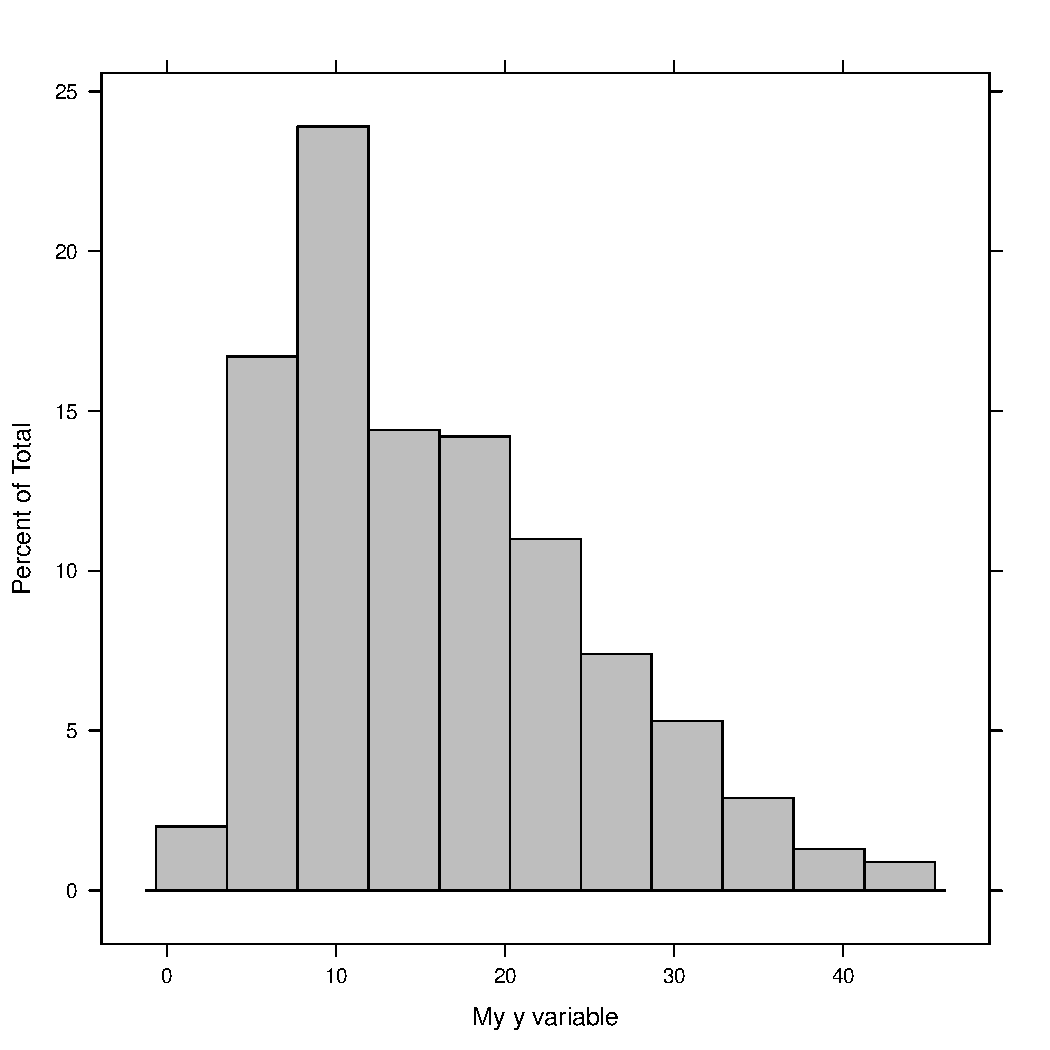
\includegraphics[width=0.6\textwidth]{../graphs/lattice_hist.pdf}
\end{frame}
\begin{frame}[fragile]
\frametitle{Histogram conditional on \texttt{x2f}}
\label{sec-2_3}


\lstset{language=R}
\begin{lstlisting}
histogram(~ y | x2f, data = df, 
          xlab = "My y variable", col = "gray")
\end{lstlisting}



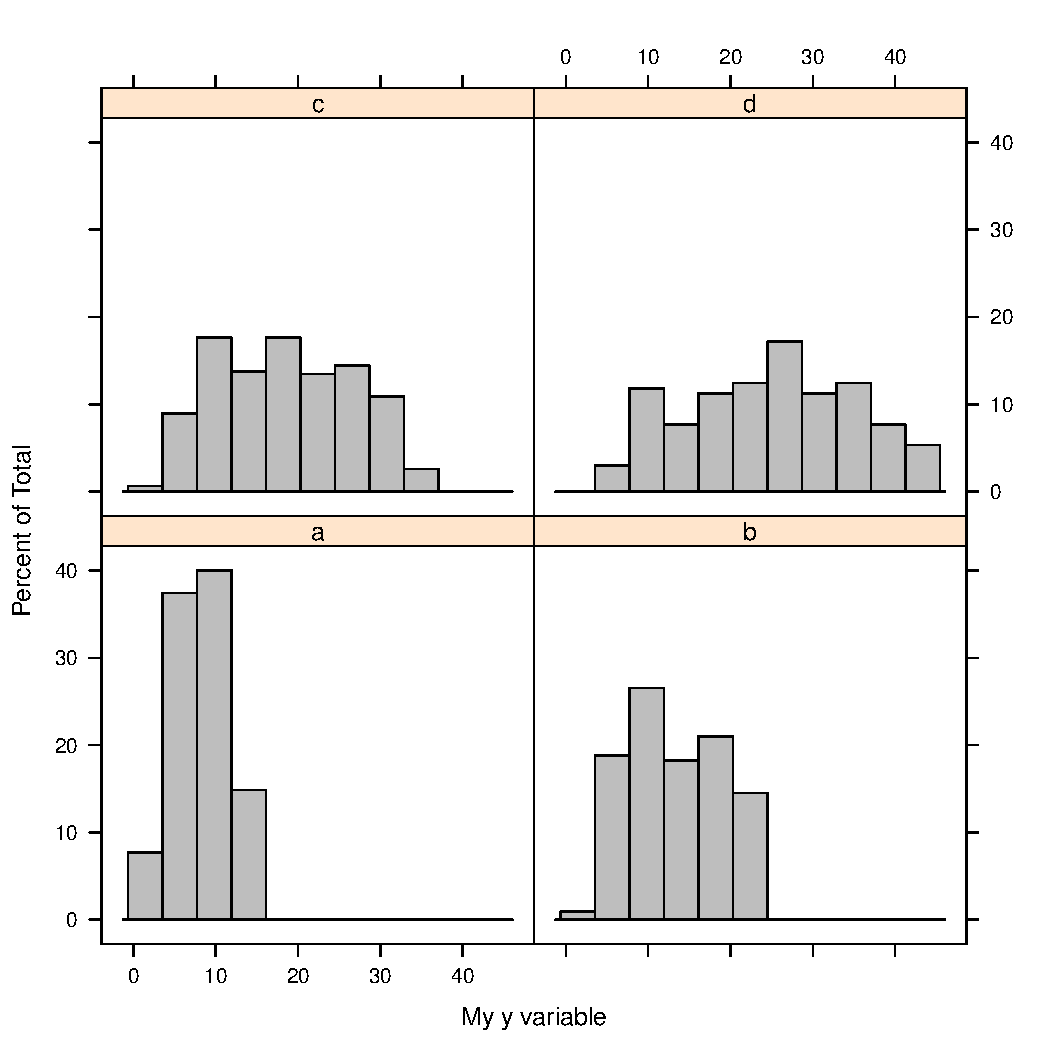
\includegraphics[width=0.6\textwidth]{../graphs/lattice_hist_g.pdf}
\end{frame}
\begin{frame}[fragile,shrink = 10]
\frametitle{Histogram with superimposed density plot}
\label{sec-2_4}

\lstset{language=R}
\begin{lstlisting}
histogram(~ y, data = df, xlab = "My y variable", 
          col = "gray", type = "density",
          panel = function(...){
              panel.histogram(...);
              panel.densityplot(..., col.line = "black")
          }
)
\end{lstlisting}



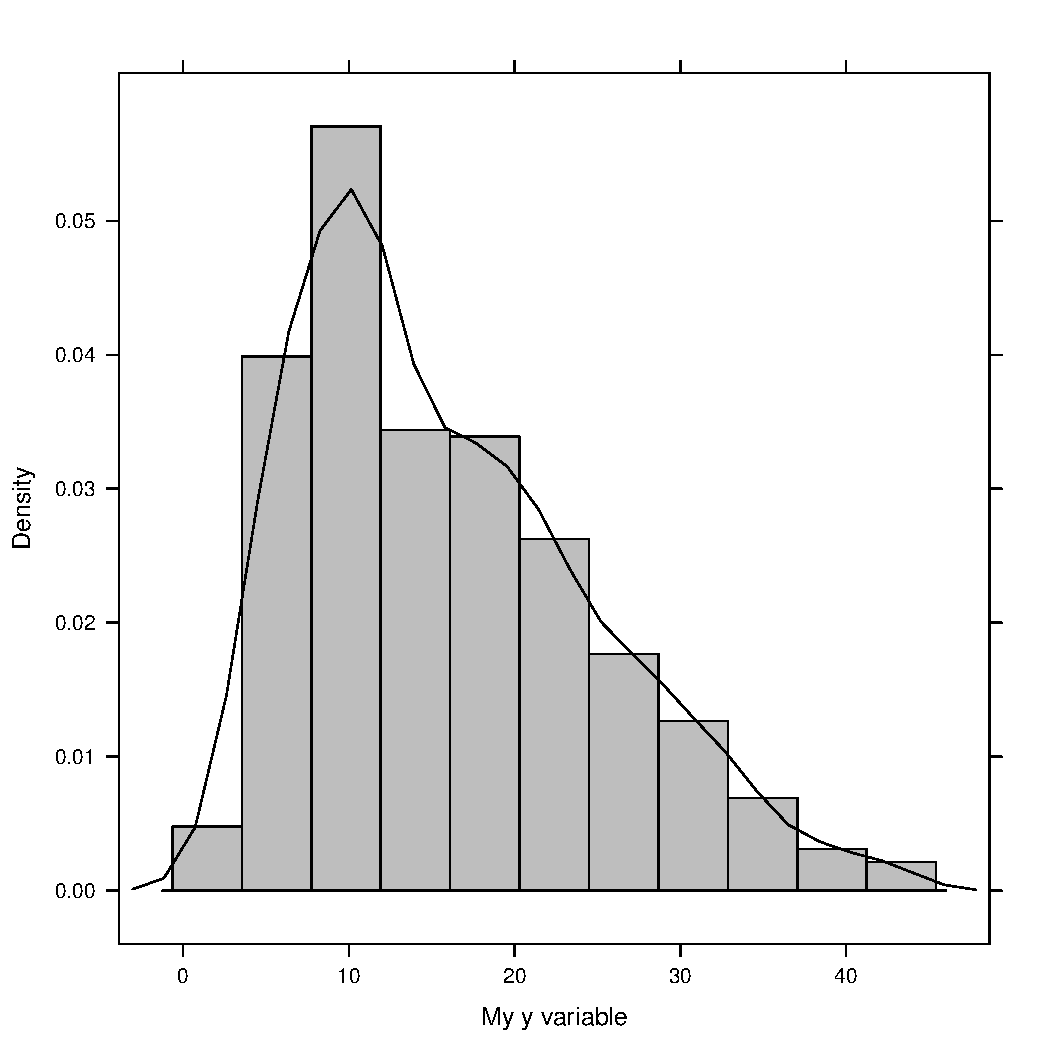
\includegraphics[width=0.6\textwidth]{../graphs/lattice_hist_dens.pdf}
\end{frame}
\begin{frame}[fragile,shrink = 10]
\frametitle{Histogram with superimposed density plot and conditional on \texttt{x2f}}
\label{sec-2_5}


\lstset{language=R}
\begin{lstlisting}
histogram(~ y | x2f, data = df, xlab = "My y variable", 
          col = "gray", type = "density",
          panel = function(...){
              panel.histogram(...);
              panel.densityplot(..., 
                                col.line = "black")
          }
)
\end{lstlisting}



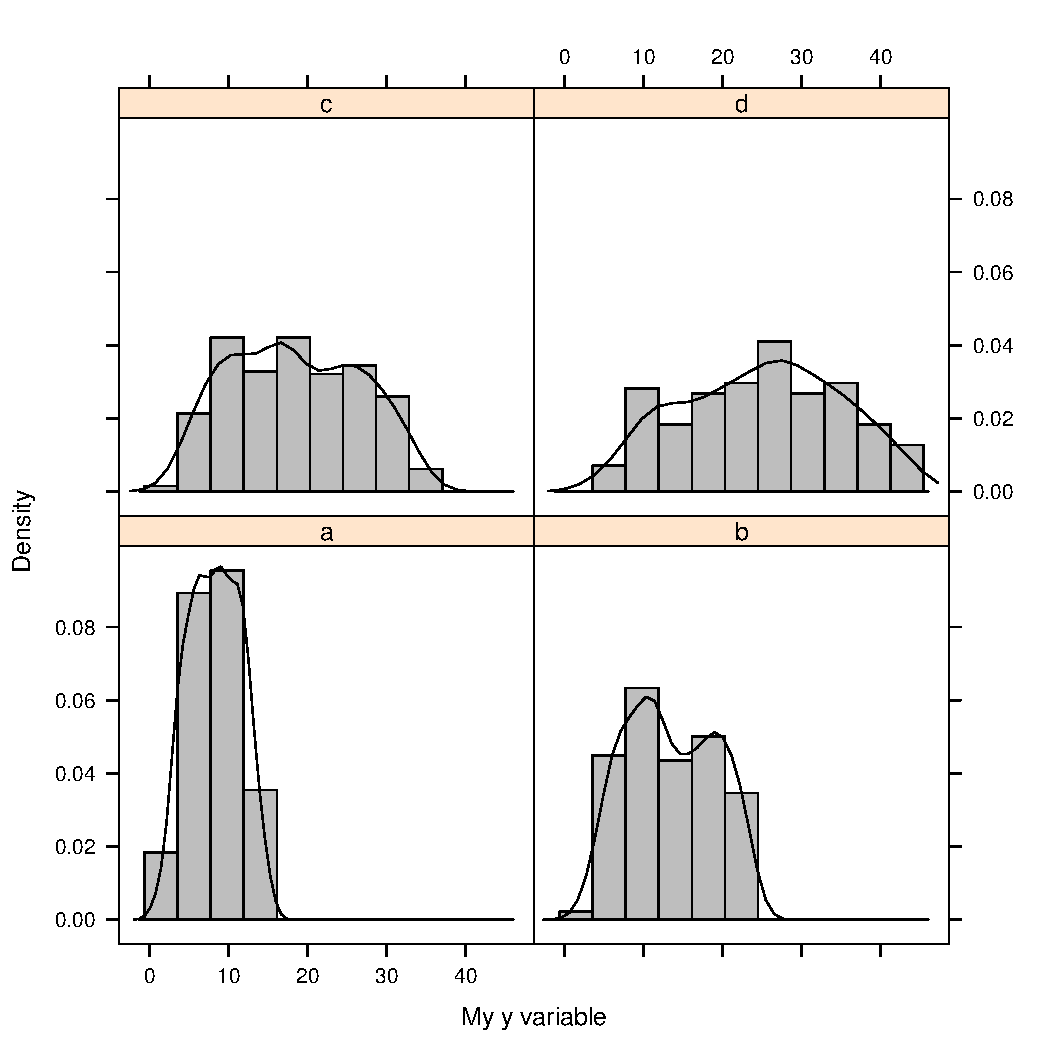
\includegraphics[width=0.6\textwidth]{../graphs/lattice_hist_dens_g.pdf}
\end{frame}
\begin{frame}[fragile]
\frametitle{Scatter plot}
\label{sec-2_6}

\lstset{language=R}
\begin{lstlisting}
xyplot(y ~ x1, data = df, 
       xlab = "My x1 variable", ylab = "My y variable")
\end{lstlisting}



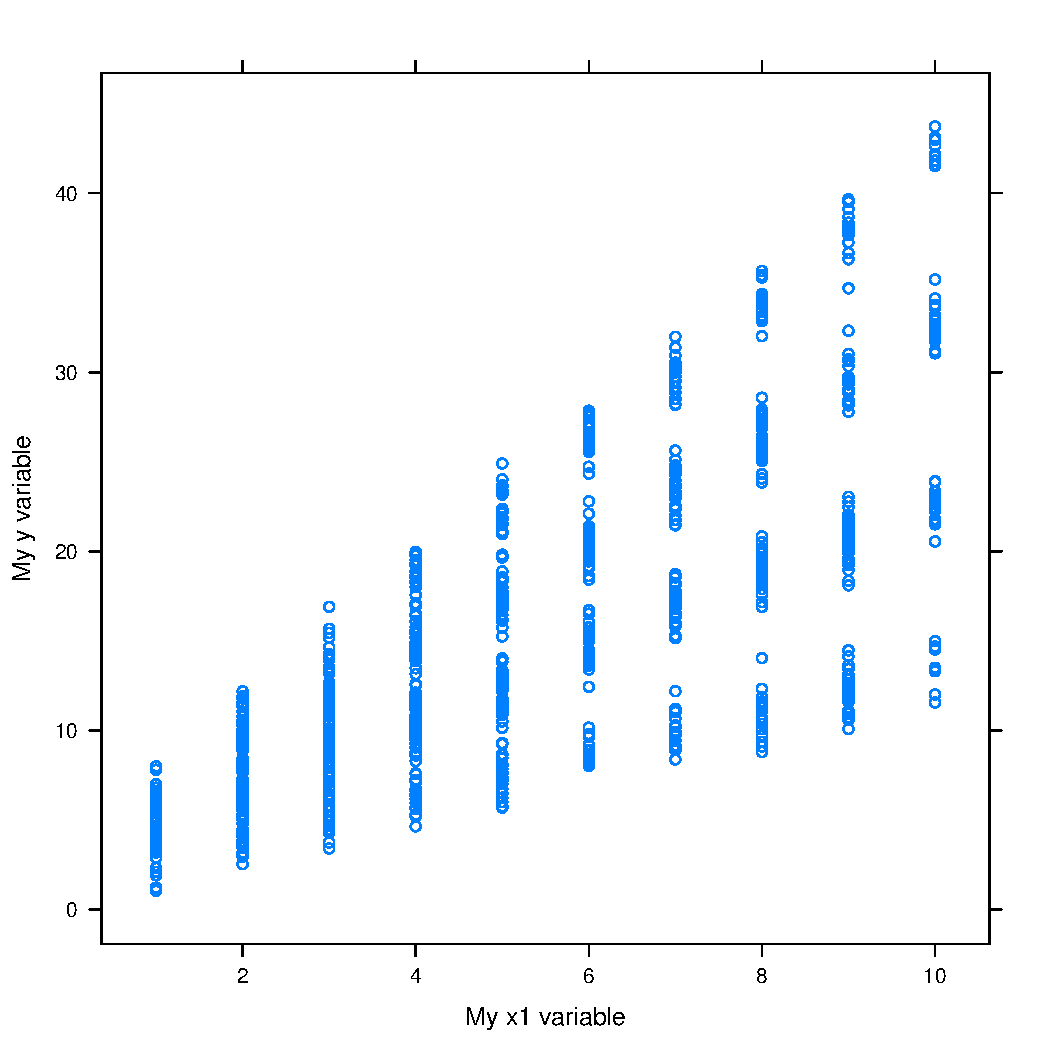
\includegraphics[width=0.6\textwidth]{../graphs/lattice_scatter.pdf}
\end{frame}
\begin{frame}[fragile]
\frametitle{Multipanel scatter plot by \texttt{x2f}}
\label{sec-2_7}

\lstset{language=R}
\begin{lstlisting}
xyplot(y ~ x1 | x2f, data = df, 
       xlab = "My x1 variable", ylab = "My y variable")
\end{lstlisting}



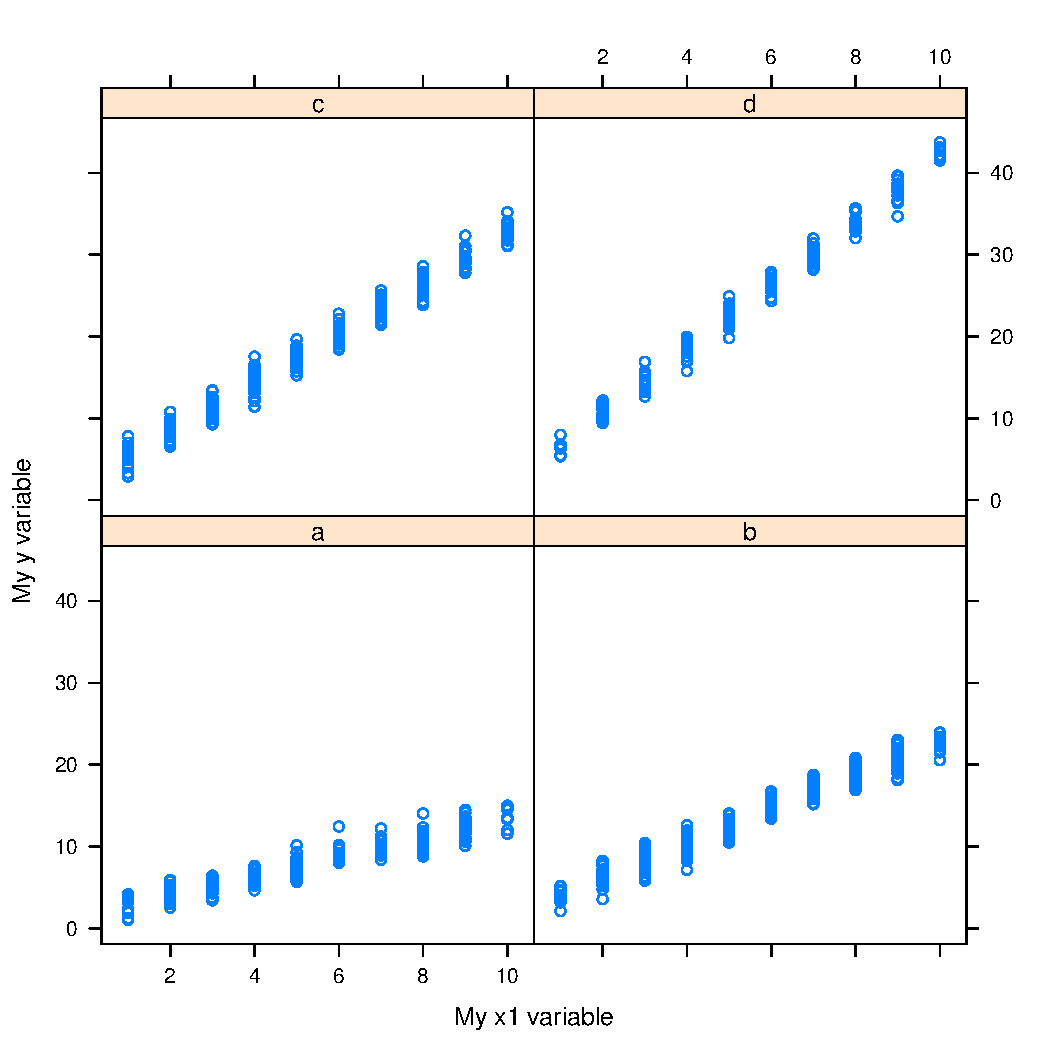
\includegraphics[width=0.6\textwidth]{../graphs/lattice_scatter_cond.pdf}
\end{frame}
\begin{frame}[fragile,shrink = 10]
\frametitle{Scatter plot by grouping variable x2}
\label{sec-2_8}

\lstset{language=R}
\begin{lstlisting}
xyplot(y ~ x1, groups = x2f, data = df,
       key = simpleKey(text = levels(df$x2f), columns = 4))
\end{lstlisting}



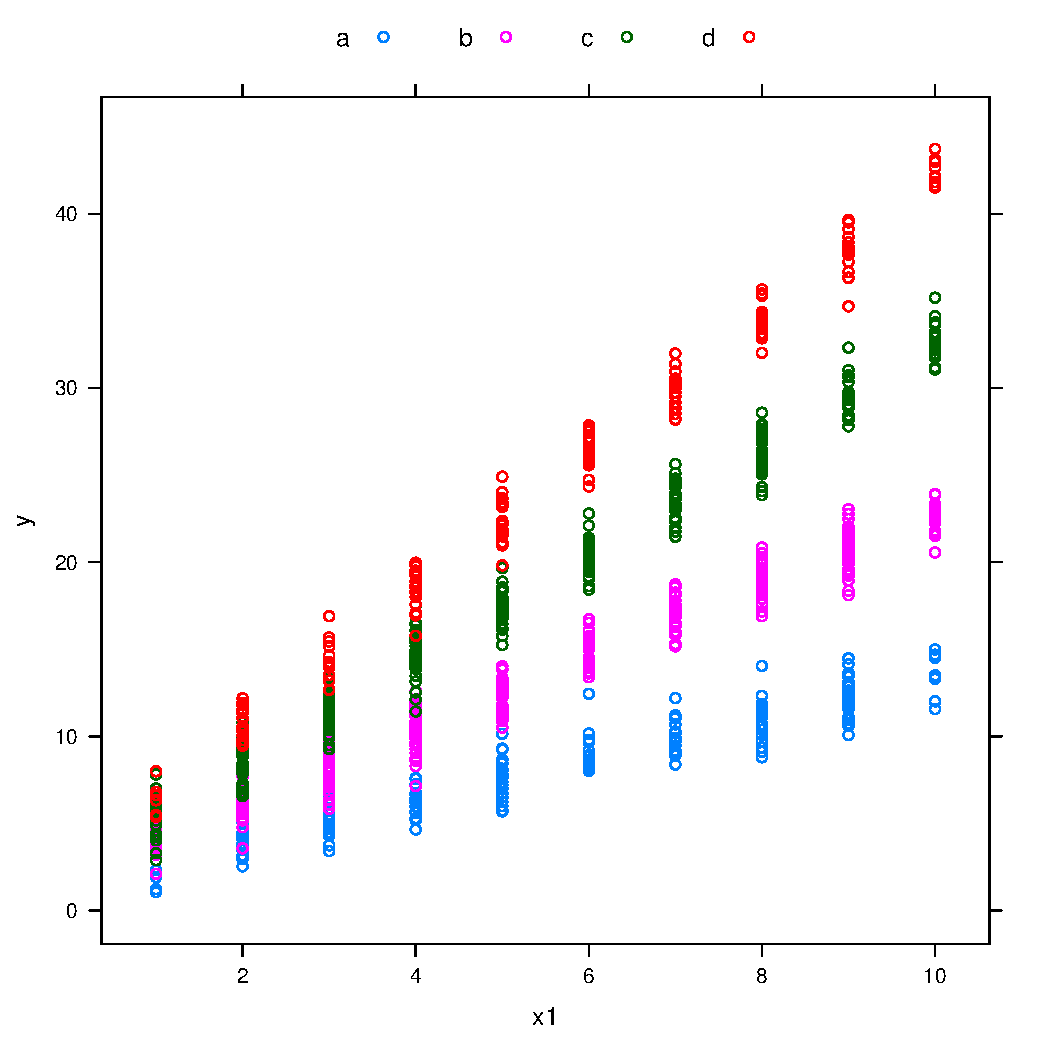
\includegraphics[width=0.6\textwidth]{../graphs/lattice_scatter_g.pdf}
\end{frame}
\begin{frame}[fragile,shrink = 10]
\frametitle{Scatter plot and linear regression line by grouping variable \texttt{x2}}
\label{sec-2_9}

\lstset{language=R}
\begin{lstlisting}
xyplot(y ~ x1 | x2, data = df, 
       panel = function(y, x1, ...){
           panel.xyplot(x1, y);
           panel.lmline(x1, y)
       })
\end{lstlisting}



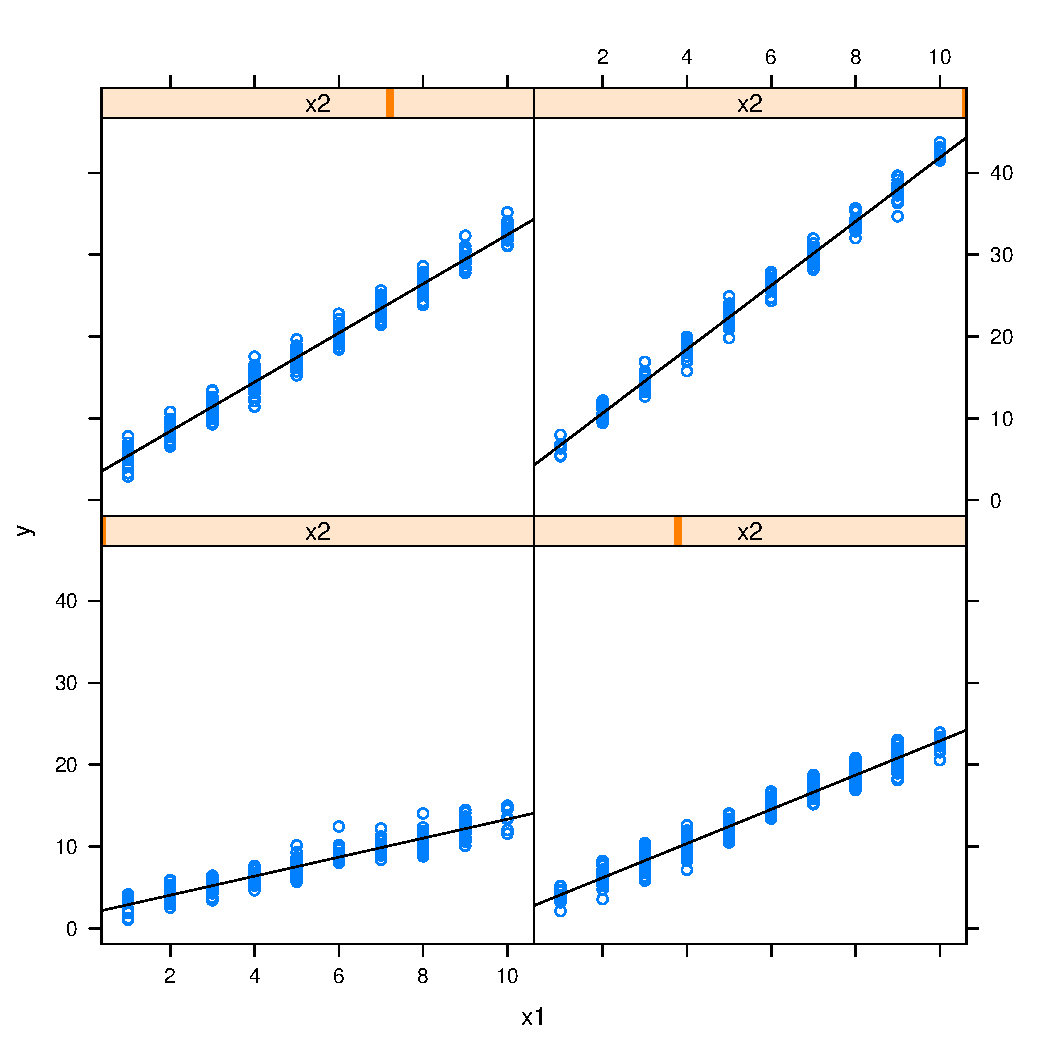
\includegraphics[width=0.6\textwidth]{../graphs/lattice_scatter_reg.pdf}
\end{frame}
\begin{frame}[fragile,shrink = 10]
\frametitle{Scatter plot and LOESS line by grouping variable \texttt{x2}}
\label{sec-2_10}

\lstset{language=R}
\begin{lstlisting}
xyplot(y ~ x1 | x2, 
       data = data.frame(df[, -2], x1 = df$x1^2), 
       panel = function(y, x1, ...){
           panel.xyplot(x1, y);
           panel.loess(x1, y)
       })
\end{lstlisting}



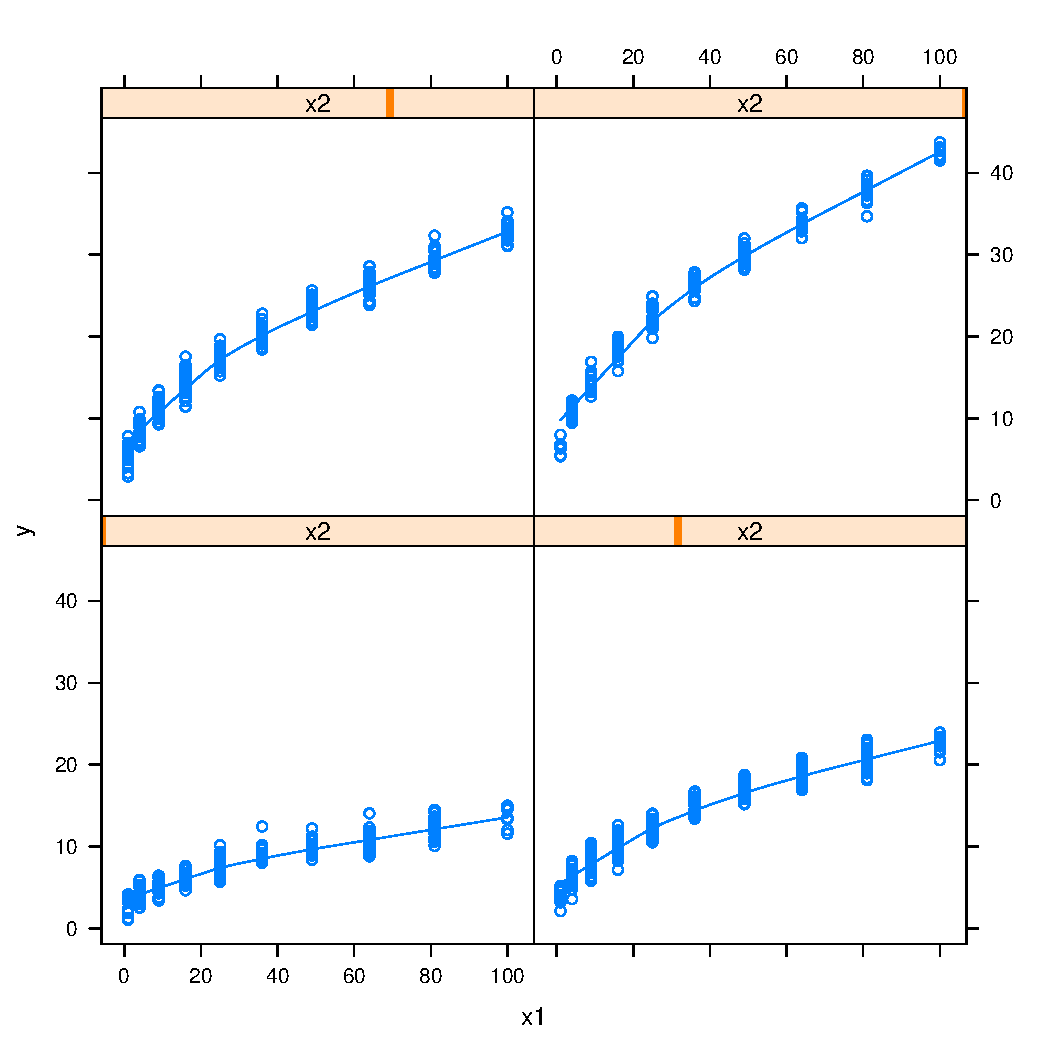
\includegraphics[width=0.6\textwidth]{../graphs/lattice_scatter_loess.pdf}
\end{frame}
\begin{frame}[fragile,shrink = 10]
\frametitle{Bar chart (absolute frequencies)}
\label{sec-2_11}

\lstset{language=R}
\begin{lstlisting}
barchart(Freq ~ Var1, data = data.frame(table(df$x2f)), 
         xlab = "My x1 variable as a factor", ylab = "N",
         col = "gray")
\end{lstlisting}



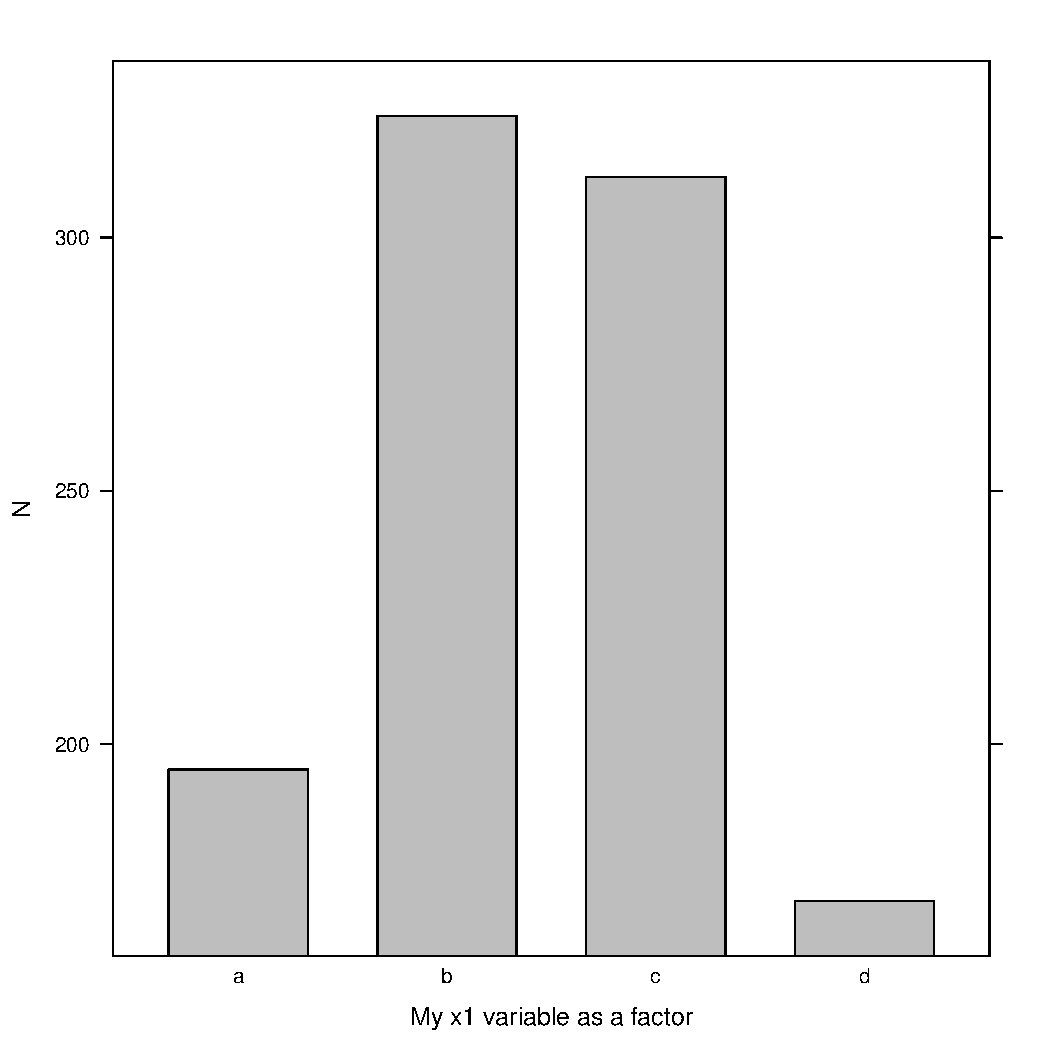
\includegraphics[width=0.6\textwidth]{../graphs/lattice_barchart_n.pdf}
\end{frame}
\begin{frame}[fragile,shrink = 10]
\frametitle{Bar chart (percentages)}
\label{sec-2_12}

\lstset{language=R}
\begin{lstlisting}
barchart(Freq ~ Var1, 
         data = data.frame(100 * prop.table(table(df$x2f))), 
         xlab = "My x1 variable as a factor", ylab = "%", 
         col = "gray")
\end{lstlisting}



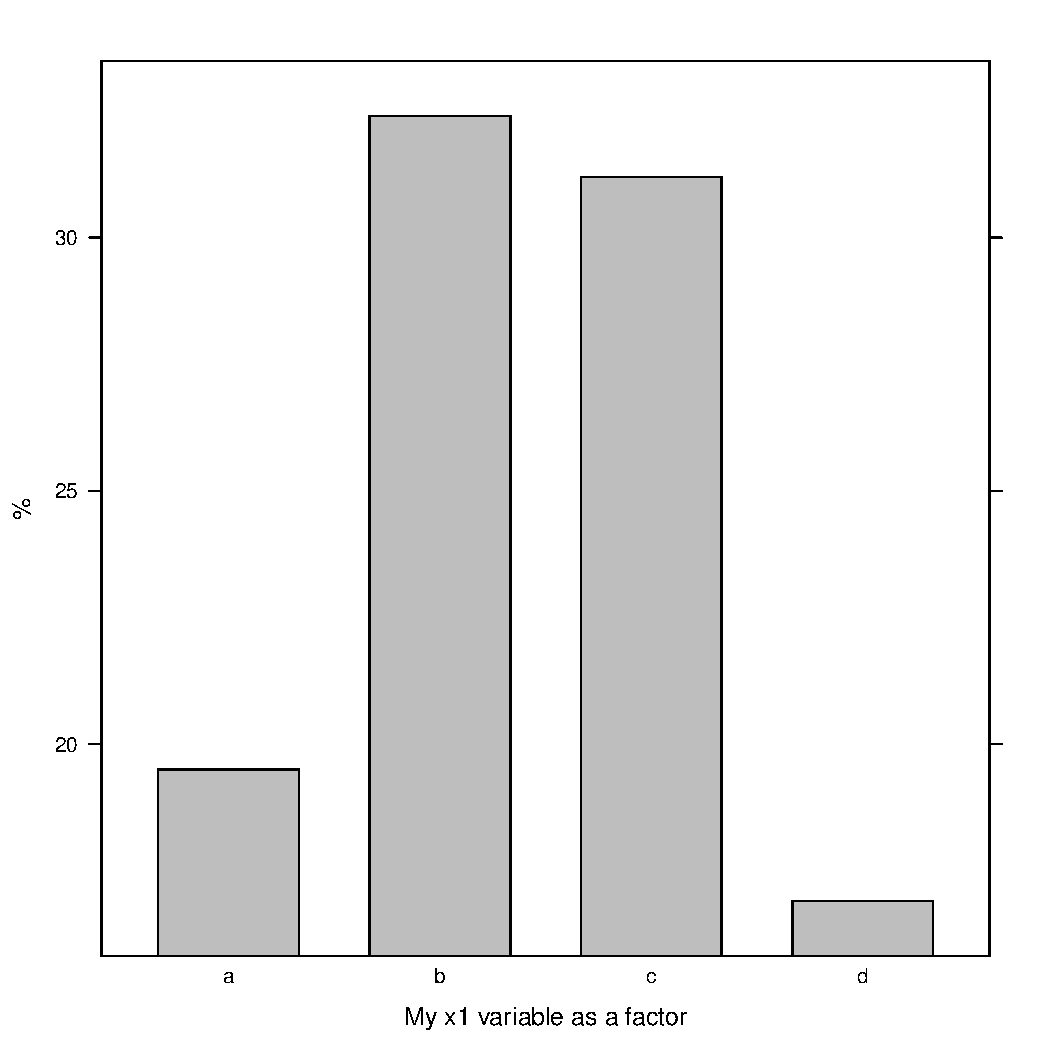
\includegraphics[width=0.6\textwidth]{../graphs/lattice_barchart_p.pdf}
\end{frame}
\begin{frame}[fragile,shrink = 10]
\frametitle{Bar chart with superimposed line plot}
\label{sec-2_13}

\lstset{language=R}
\begin{lstlisting}
barchart(Freq ~ Var1, data = data.frame(table(df$x2f)), 
         xlab = "My x1 variable as a factor", ylab = "N",
         col = "gray",
         panel = function(...){
             panel.barchart(...);
             panel.xyplot(..., type = "b", col.symbol = "red", 
                          col.line = "red");
         })
\end{lstlisting}



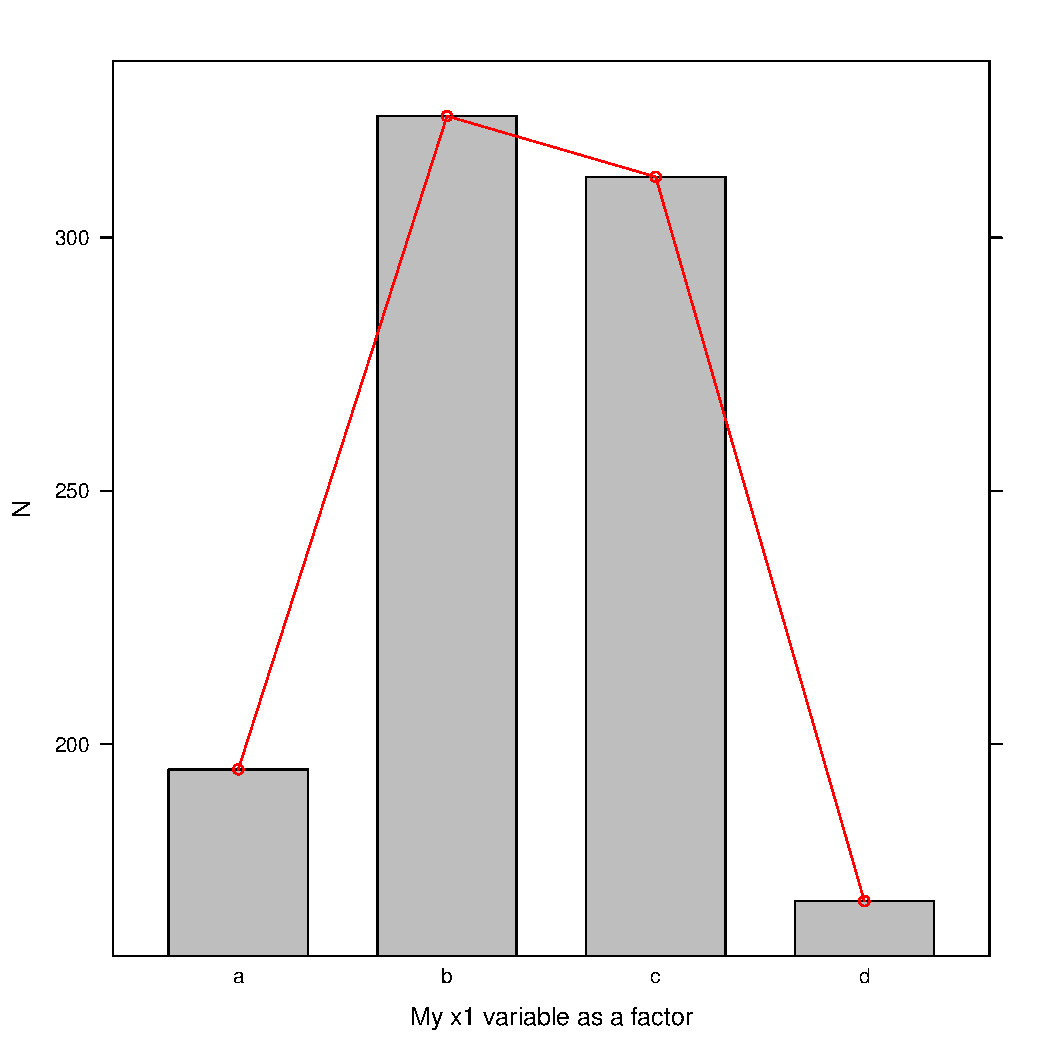
\includegraphics[width=0.55\textwidth]{../graphs/lattice_barchart_lines.pdf}
\end{frame}
\section{The ggplot2 package}
\label{sec-3}
\begin{frame}[shrink = 10]
\frametitle{A basic overview about the ggplot2 package}
\label{sec-3_1}


\begin{itemize}
\item Needs to be loaded via \texttt{library(ggplot2)}
\item Is based on The Grammar of Graphics by Leland Wilkinson
\item Sometimes difficult to ``tweak'' plots which do not follow the GoG (and Hadley Wickham's
  implementation of the GoG)
\item Often, original data need to be modified (e.g., aggregated for barcharts)
\item Web resources:

\begin{itemize}
\item \href{http://had.co.nz/ggplot2/}{Hadley Wickham's website for ggplot2} (this website is simply awesome; he also has
    written a ggplot2 related book)
\item \href{https://github.com/hadley/ggplot2/wiki}{Wiki for ggplot2: Elegant graphics for data analysis} (ultimate resource when it comes to fine tuning)
\item \href{http://learnr.wordpress.com/}{The blog Learning R offers a lot of examples of how ggplot2 works}
\item Visualizing Data with R and ggplot2 (video w/ slides) (website: www.drewconway.com/zia/?p=1637)
\end{itemize}

\end{itemize}
\end{frame}
\begin{frame}[fragile]
\frametitle{Histogram}
\label{sec-3_2}


\lstset{language=R}
\begin{lstlisting}
ggplot(aes(x = y), data = df) + geom_histogram() + 
    xlab("My y variable") + ylab("N")
\end{lstlisting}



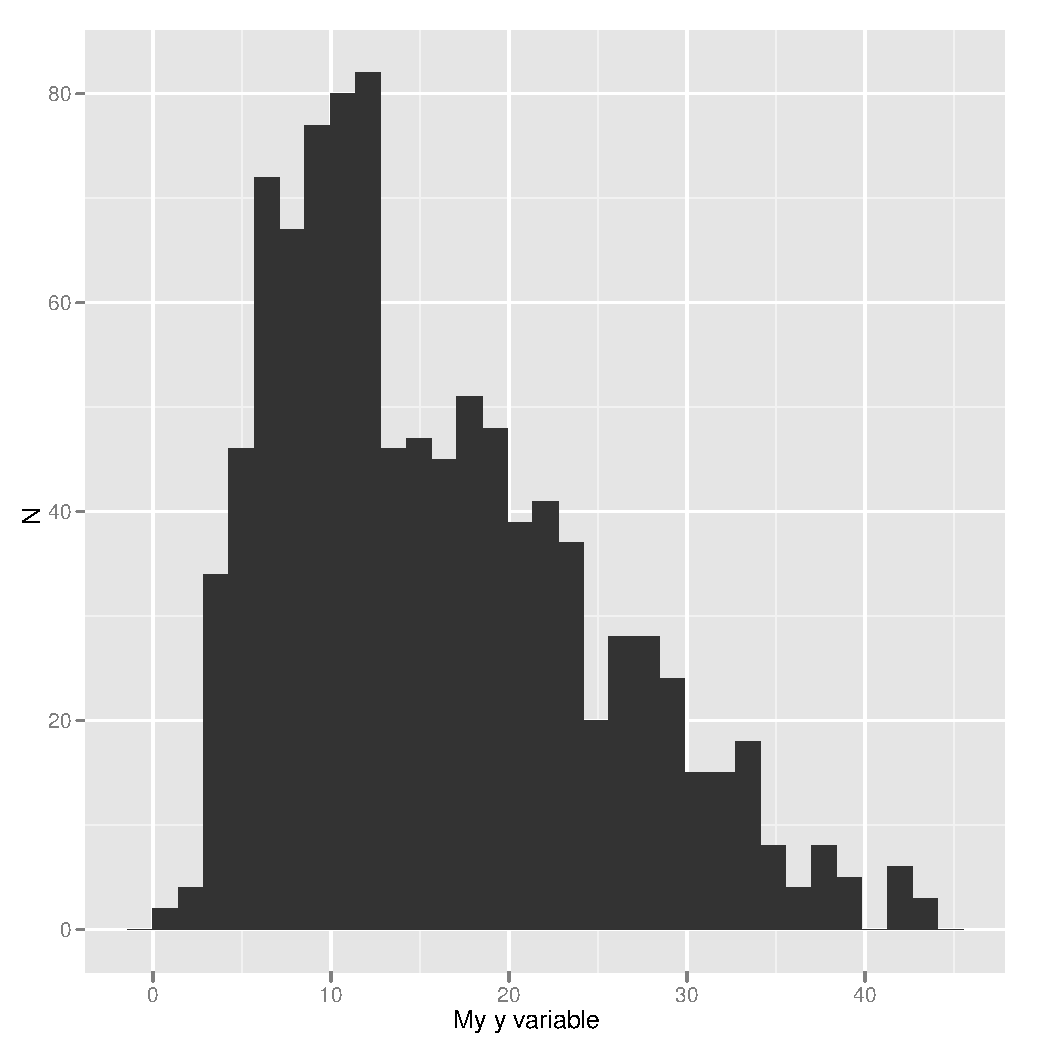
\includegraphics[width=0.6\textwidth]{../graphs/ggplot2_hist.pdf}
\end{frame}
\begin{frame}[fragile]
\frametitle{Histogram conditional on \texttt{x2f}}
\label{sec-3_3}


\lstset{language=R}
\begin{lstlisting}
ggplot(aes(x = y), data = df) + geom_histogram() + 
    xlab("My y variable") + ylab("N") + facet_wrap(~x2f)
\end{lstlisting}



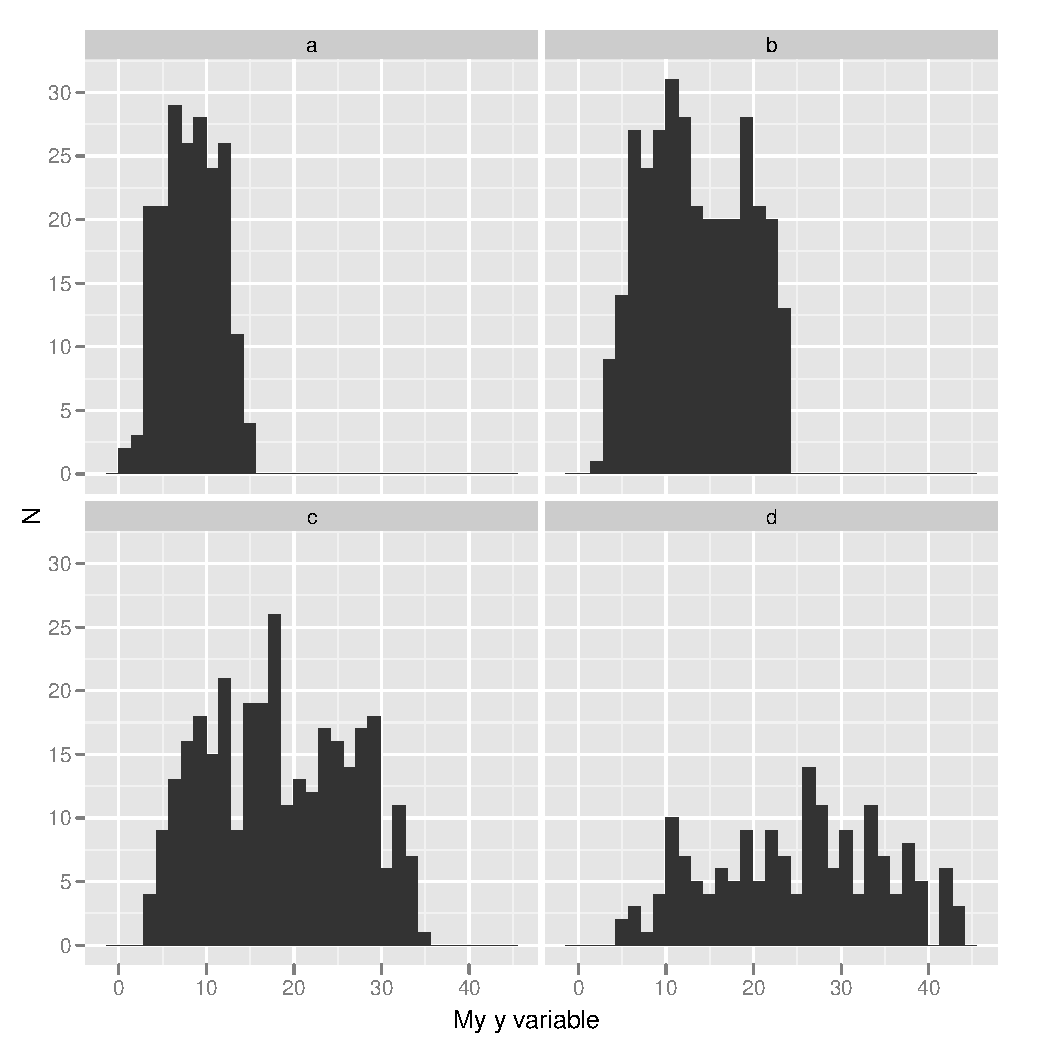
\includegraphics[width=0.6\textwidth]{../graphs/ggplot2_hist_g.pdf}
\end{frame}
\begin{frame}[fragile,shrink = 10]
\frametitle{Histogram with superimposed density plot and conditional on \texttt{x2f}}
\label{sec-3_4}

\lstset{language=R}
\begin{lstlisting}
ggplot(aes(x = y), data = df) + 
    geom_histogram(aes(y = ..density..)) + 
    geom_density(colour = "grey", size = 1.2) + 
    xlab("My y variable") + ylab("N") + 
    facet_wrap(~x2f)
\end{lstlisting}



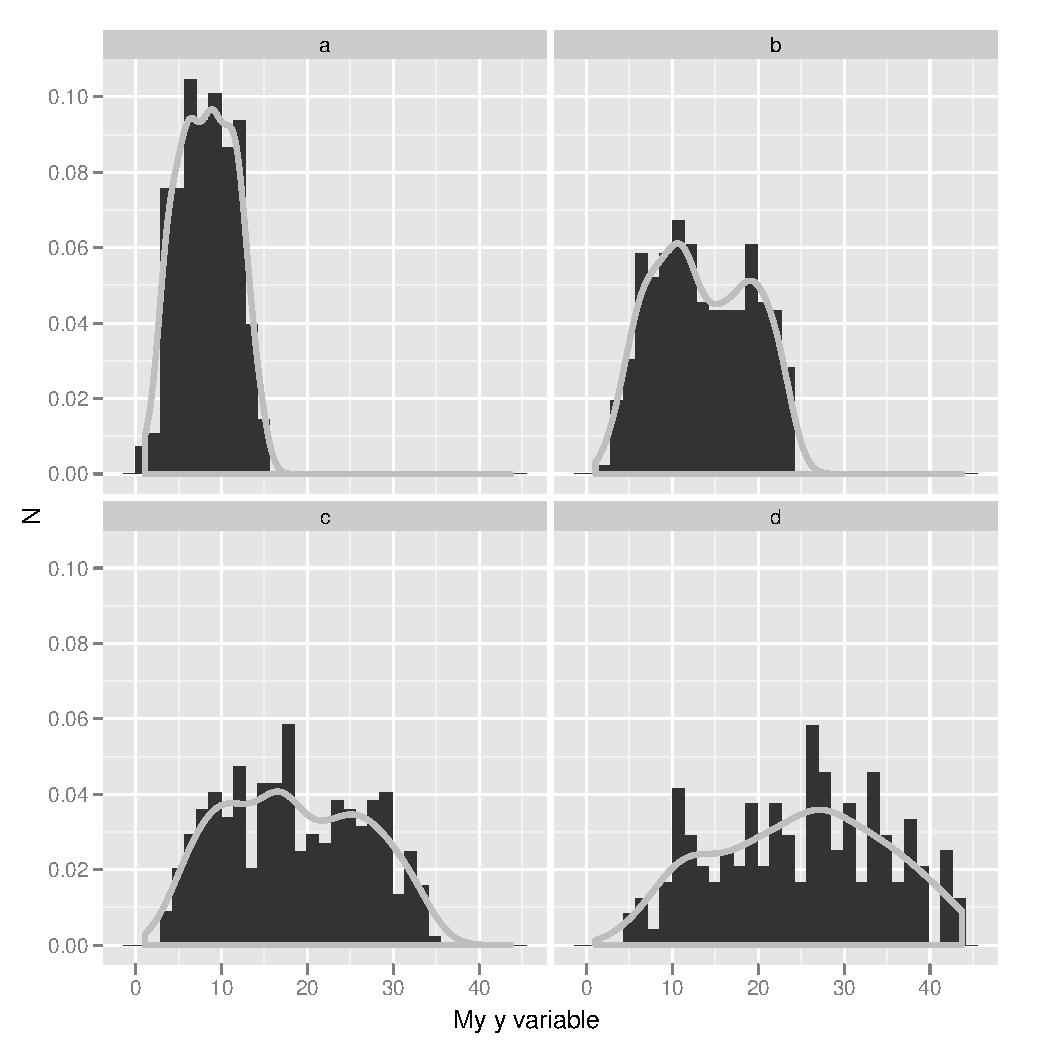
\includegraphics[width=0.6\textwidth]{../graphs/ggplot2_hist_dens.pdf}
\end{frame}
\begin{frame}[fragile]
\frametitle{Scatter plot}
\label{sec-3_5}

\lstset{language=R}
\begin{lstlisting}
ggplot(aes(x = x1, y = y), data = df) + geom_point() + 
    xlab("My x1 variable") + ylab("My y variable")
\end{lstlisting}



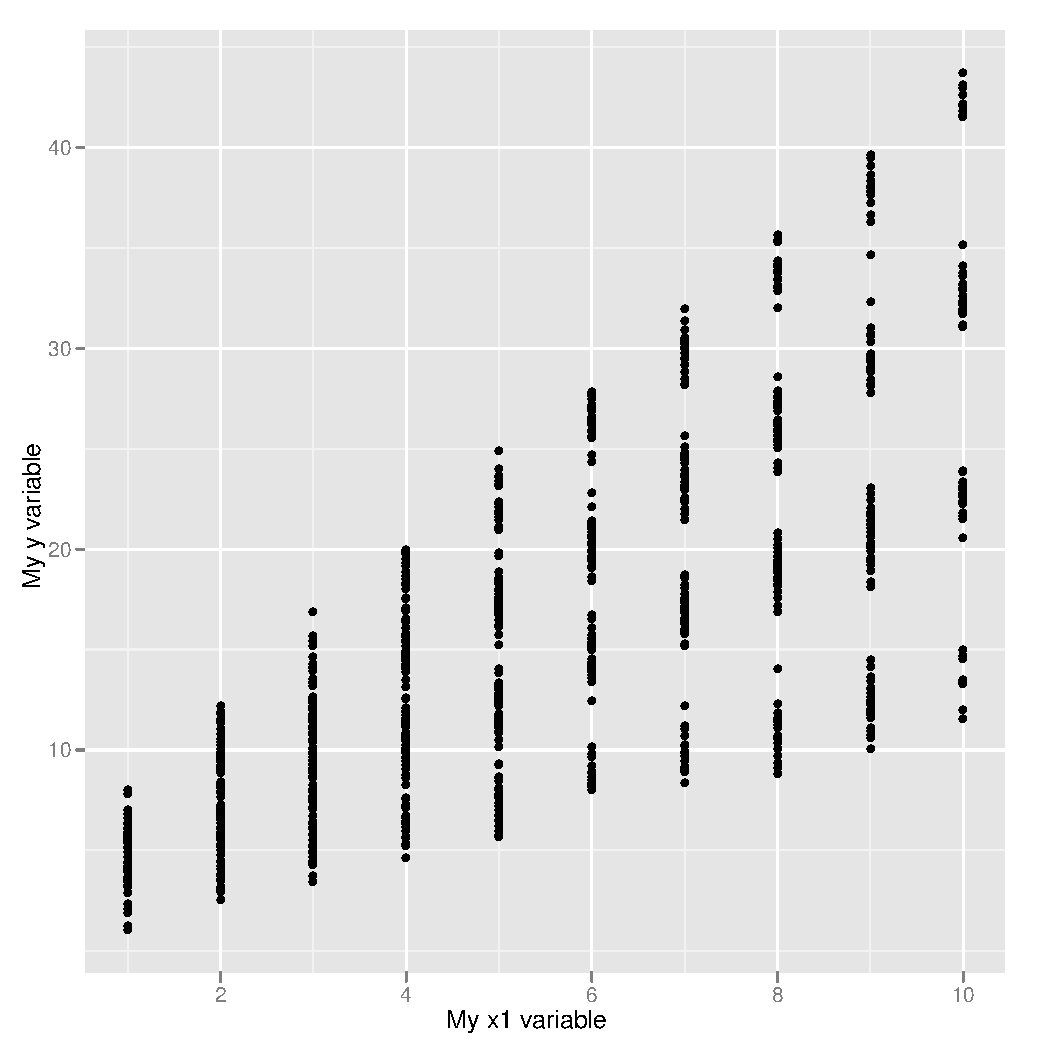
\includegraphics[width=0.6\textwidth]{../graphs/ggplot2_scatter.pdf}
\end{frame}
\begin{frame}[fragile]
\frametitle{Multipanel scatter plot by \texttt{x2f}}
\label{sec-3_6}

\lstset{language=R}
\begin{lstlisting}
ggplot(aes(x = x1, y = y), data = df) + geom_point() + 
    xlab("My x1 variable") + ylab("My y variable") +
    facet_wrap(~ x2f)
\end{lstlisting}



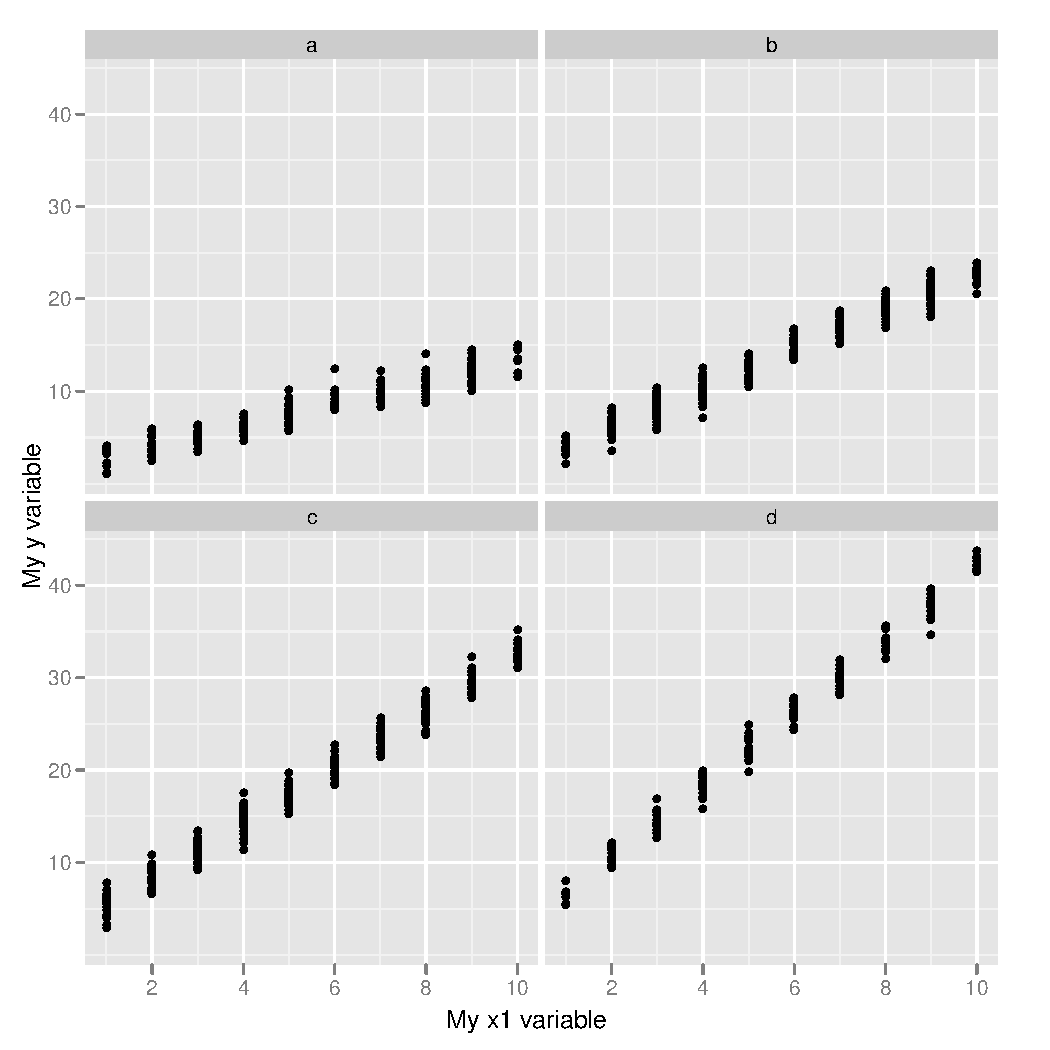
\includegraphics[width=0.6\textwidth]{../graphs/ggplot2_scatter_cond.pdf}
\end{frame}
\begin{frame}[fragile,shrink = 10]
\frametitle{Scatter plot by grouping variable x2}
\label{sec-3_7}

\lstset{language=R}
\begin{lstlisting}
ggplot(aes(x = x1, y = y, colour = x2f), data = df) + 
    geom_point() + xlab("My x1 variable") + 
    ylab("My y variable")
\end{lstlisting}



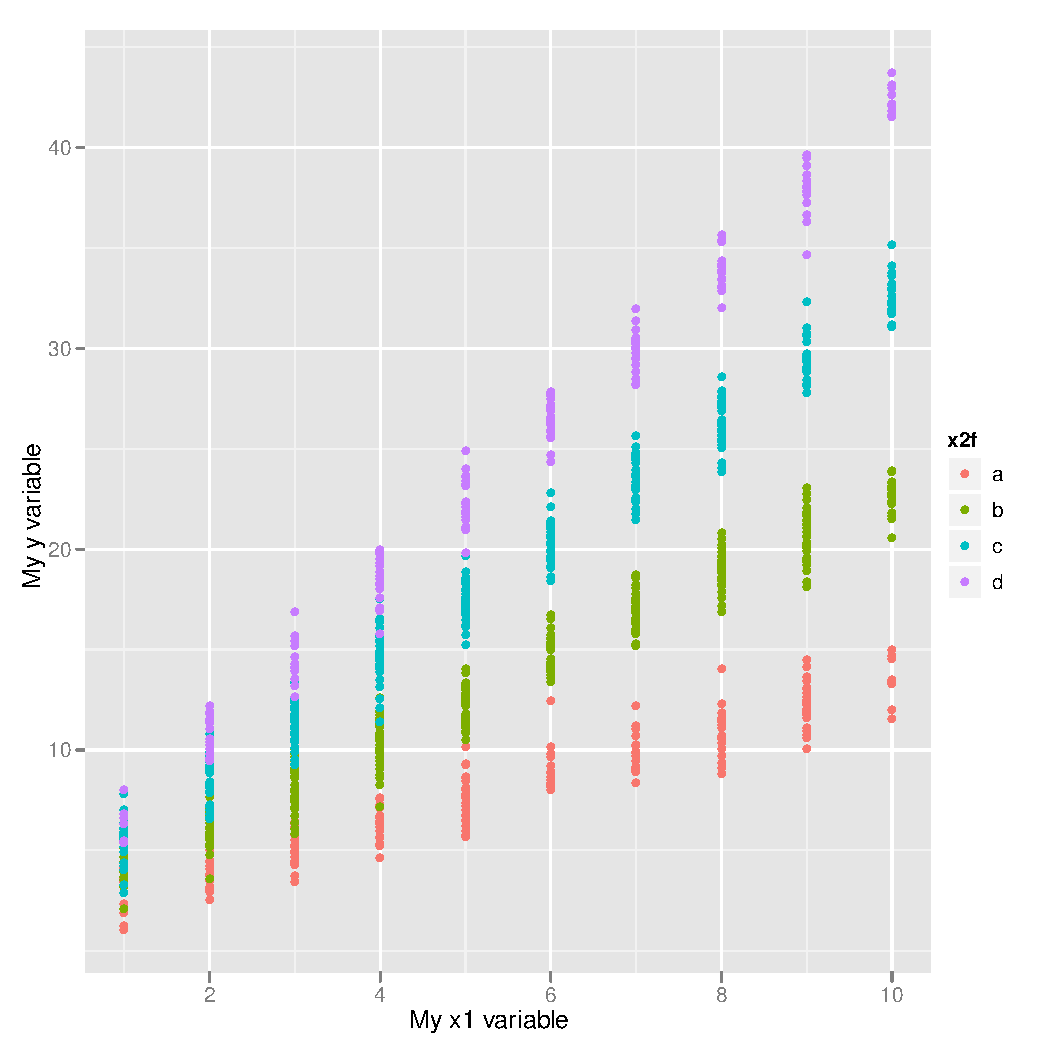
\includegraphics[width=0.6\textwidth]{../graphs/ggplot2_scatter_g.pdf}
\end{frame}
\begin{frame}[fragile,shrink = 15]
\frametitle{Scatter plot and linear regression line by \texttt{x2}}
\label{sec-3_8}

\lstset{language=R}
\begin{lstlisting}
ggplot(aes(x = x1, y = y, colour = x2f), data = df) + 
    geom_point() + xlab("My x1 variable") + 
    ylab("My y variable") + facet_wrap(~x2f) +
    geom_smooth(method = "lm")
\end{lstlisting}



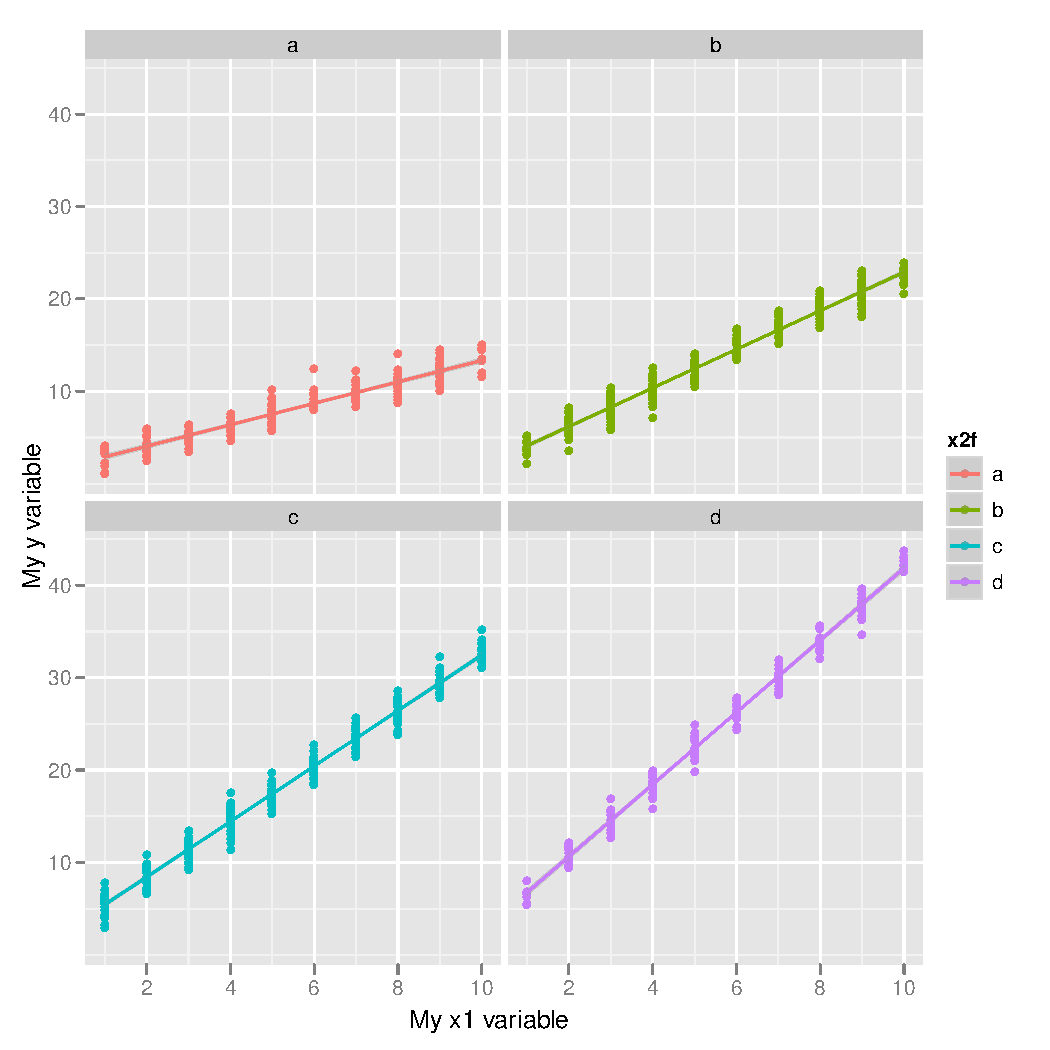
\includegraphics[width=0.6\textwidth]{../graphs/ggplot2_scatter_reg.pdf}
\end{frame}
\begin{frame}[fragile,shrink = 10]
\frametitle{Scatter plot and LOESS line by \texttt{x2}}
\label{sec-3_9}

\lstset{language=R}
\begin{lstlisting}
ggplot(aes(x = x1, y = y, colour = x2f), 
       data = data.frame(df[, -2], x1 = df$x1^2)) + 
    geom_point() + xlab("My x1 variable") + 
    ylab("My y variable") + facet_wrap(~x2f) +
    geom_smooth(method = "loess")
\end{lstlisting}



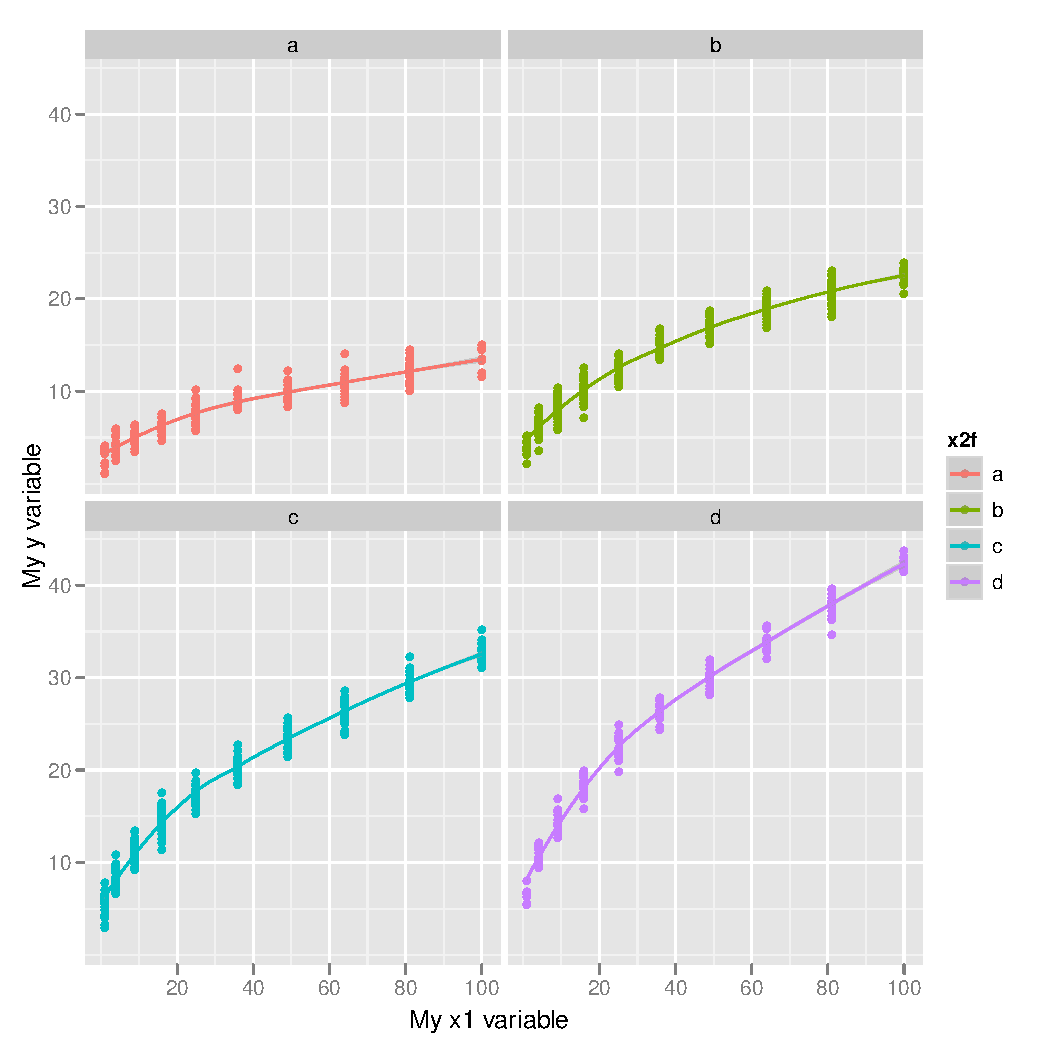
\includegraphics[width=0.6\textwidth]{../graphs/ggplot2_scatter_loess.pdf}
\end{frame}
\begin{frame}[fragile,shrink = 10]
\frametitle{Bar chart (absolute frequencies)}
\label{sec-3_10}

\lstset{language=R}
\begin{lstlisting}
ggplot(aes(x = x2f), data = df) + geom_bar(fill = "red")
\end{lstlisting}



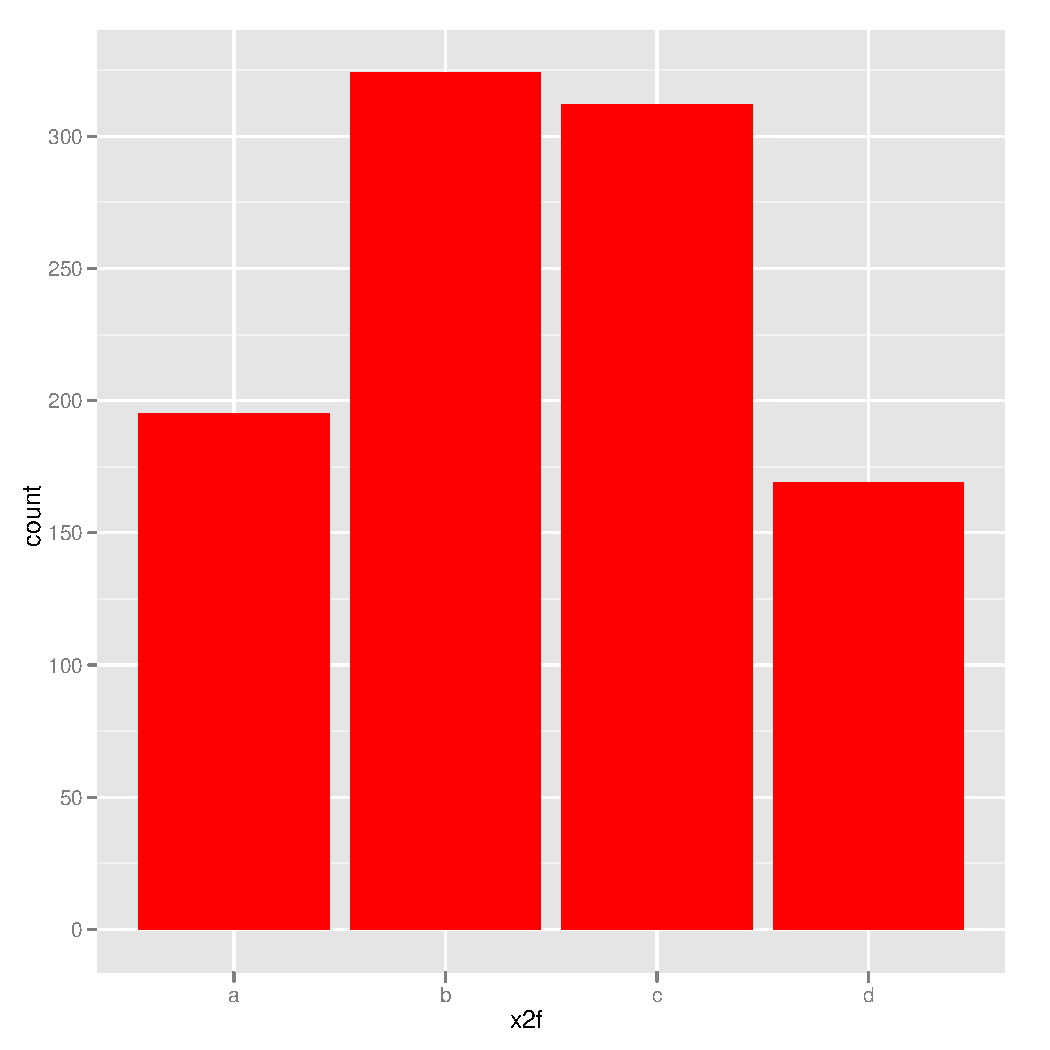
\includegraphics[width=0.6\textwidth]{../graphs/ggplot2_barchart_n.pdf}
\end{frame}
\begin{frame}[fragile,shrink = 10]
\frametitle{Bar chart (percentages)}
\label{sec-3_11}

\lstset{language=R}
\begin{lstlisting}
tmp <- data.frame(prop.table(table(df$x2f)))
ggplot(aes(x = Var1, y = Freq), data = tmp) + 
    geom_bar(fill = "red")
\end{lstlisting}



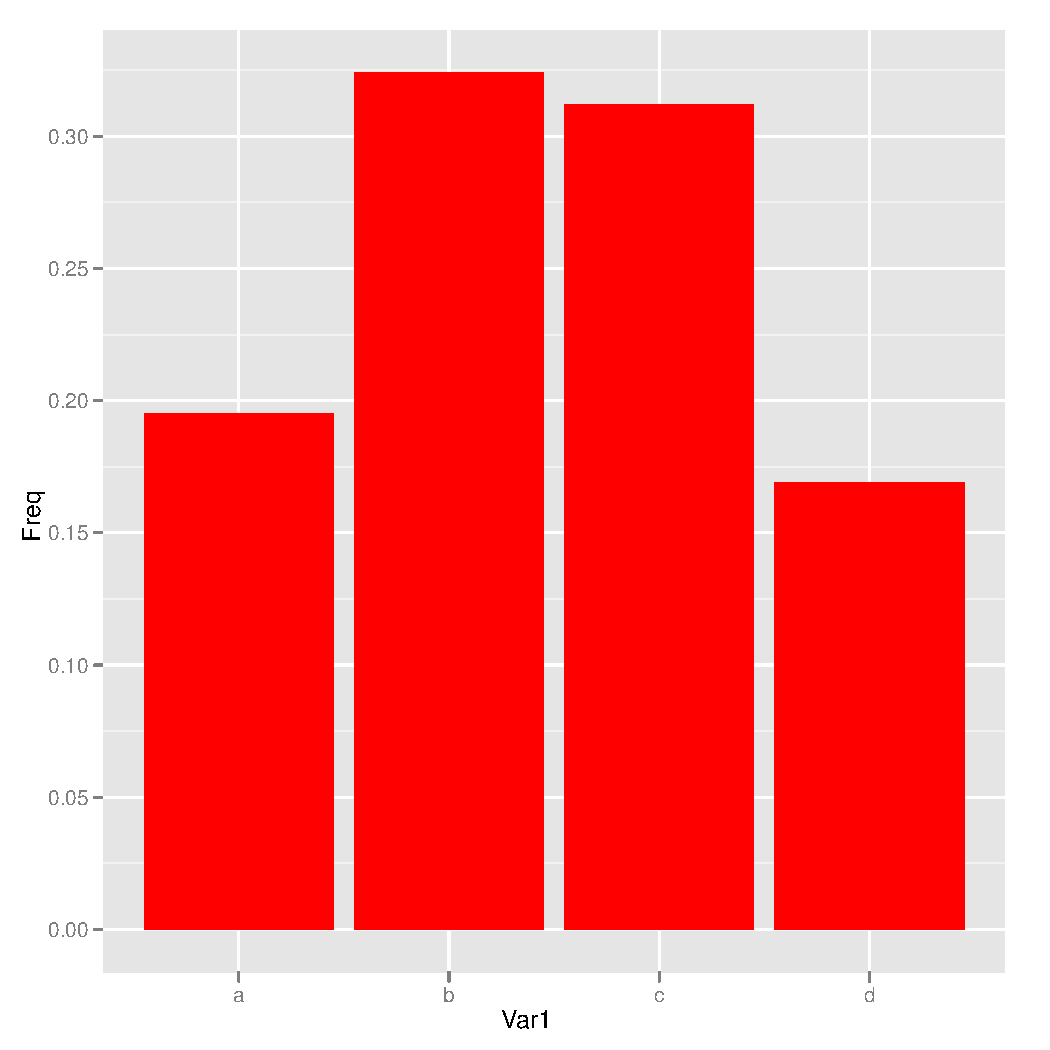
\includegraphics[width=0.6\textwidth]{../graphs/ggplot2_barchart_p.pdf}
\end{frame}
\begin{frame}[fragile,shrink = 10]
\frametitle{Box plot, jittered scatterplot, LOESS line (slightly useless\ldots)}
\label{sec-3_12}

\lstset{language=R}
\begin{lstlisting}
ggplot(aes(x = x2f, y = y), data = df) +
    geom_jitter() + geom_boxplot(alpha = 0.8) + 
    stat_smooth(aes(x = as.numeric(x2f, y = y)), 
                data = df, method = "loess", 
                level = 0.90) + 
    geom_hline(yintercept = mean(df$y), 
               col = "green", size = 1.2)
\end{lstlisting}



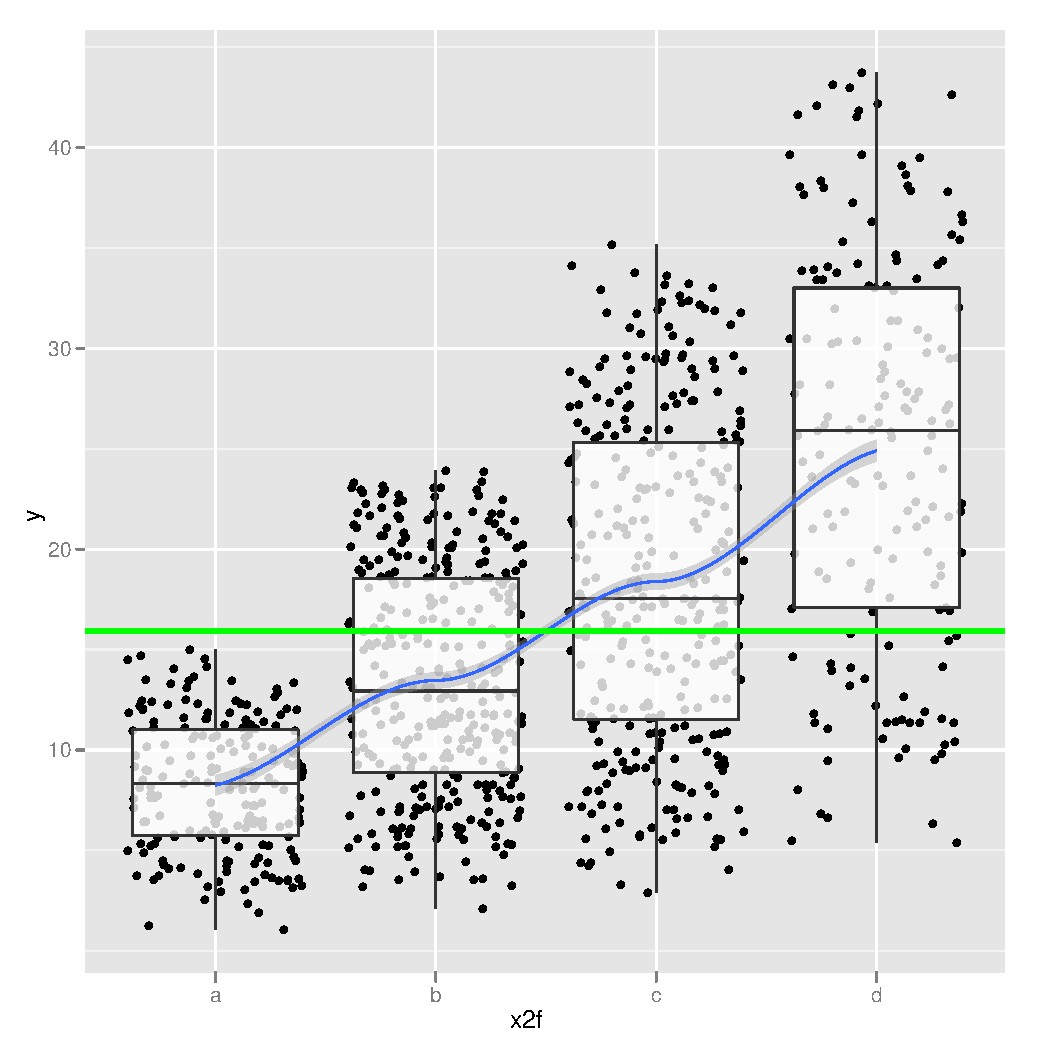
\includegraphics[width=0.6\textwidth]{../graphs/ggplot2_boxplot.pdf}


  
\end{frame}

\end{document}